\documentclass{beamer}
\usepackage{pgfpages}
%Math and symbol packages
\usepackage{amsmath}
\usepackage{amsfonts}
\usepackage{amssymb}

%Graphics
\usepackage{graphicx}
\usepackage{grffile} %Allows the graphics files to have spaces in their addresses
\usepackage{caption}
\usepackage{subcaption}

%\usepackage{titlesec} for customizing section headers

\usetheme{CambridgeUS}
\usecolortheme{rose}
\graphicspath{{../figs/}}

\title[Mg II absorbers along QSO LoS]{Distribution of Mg II absorbers in along QSO lines of sight}
\subtitle{Dual degree project: 2017-18}
\author{Sunil Simha}
\institute[IIT Madras]{Indian Institute of Technology, Madras\\Guided by\\
	\small Dr. L Sriramkumar\\ \tiny{and}\\\small Dr. R Srianand, IUCAA, Pune}
\date[26-01-2018]{26$^{th}$ January 2018}


\begin{document}
	\begin{frame}
		\titlepage
	\end{frame}
	%----------------------------------------------
	\begin{frame}{Contents}
		\tableofcontents
	\end{frame}
	%----------------------------------------------
\section{Introduction}
	\subsection{Mg II absorbers along QSO sightlines}
		\begin{frame}[allowframebreaks]{Mg II absorbers along QSO sightlines}
			\begin{figure}
				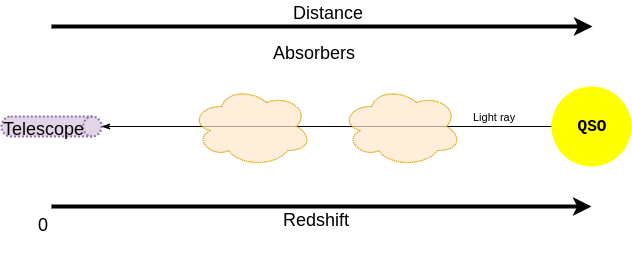
\includegraphics[width=0.8\textwidth]{system.png}
				\caption{\tiny The absorption system}
				\label{fig:system}
			\end{figure}
			\begin{itemize}
				\item\small Mg II ions have been known to be tracers of neutral gas.
				\item\small One of the strongest lines and thus easily spotted.
				\item\small Specifically looking at the doublet 2796-2803 \AA
			\end{itemize}
			\begin{figure}
				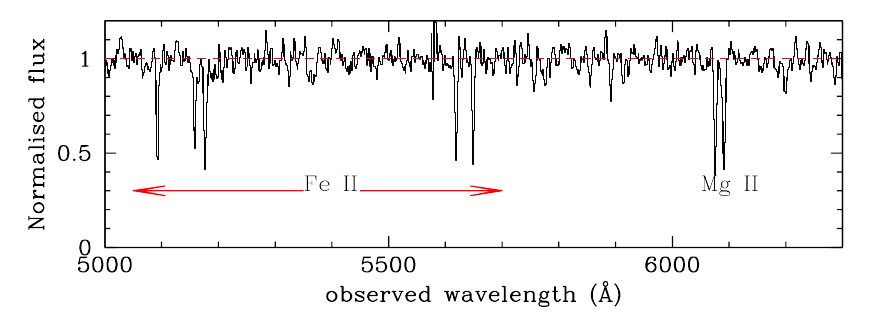
\includegraphics[width=\textwidth]{srianand-spectrum.png}
				\caption{\tiny Mg II absorbers in QSO spectrum. Note the wavelength of the Mg II lines. They have been redshifted to nearly 6100 \AA from their rest wavelength of 2800 \AA. \emph{Source: R. Srianand, private communication}}
			\end{figure}
				%	\begin{block}{QSOs as probes}
				%		\begin{itemize}
				%			\item QSOs can serve as a good background source. Very distant
				%			\item Broad-band emission. Absorption can happen at different wavelengths
				%			\item Numerous. Can probe a large area of the sky.
				%		\end{itemize}
				%	\end{block}
		\end{frame}
		\begin{frame}{QSO sightlines}
			\begin{figure}
				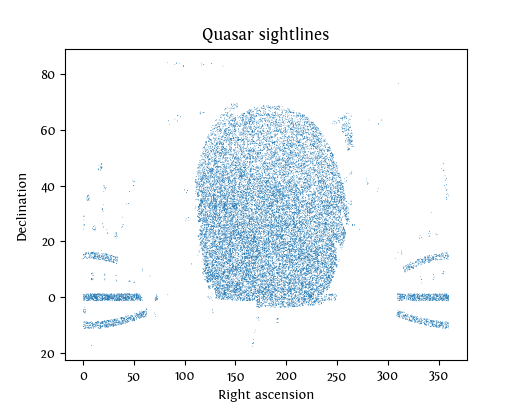
\includegraphics[width=0.7\textwidth]{qso_sky.png}
				\caption{\tiny All QSO sightlines considered}
				\label{fig:QSOs}
			\end{figure}
		\end{frame}
		\begin{frame}{Goals of this project}
			\begin{itemize}
				\item To study the distribution of Mg II absorbers in redshift space
				\item To model this distribution and hence make inferences on the distribution of dark matter halos
			\end{itemize}
			Understanding the relationship between cold gas and dark matter halos would help understand structure formation better.
			\begin{block}{Work in progress}
				Modelling the distribution of absorbers
			\end{block}
			\begin{block}{Work to be done}
				Modelling the \textbf{clustering} of absorbers as well
			\end{block}
		\end{frame}
%--------------------------------------------------
\section{Theory}
\subsection{Cosmological perturbation theory}
\begin{frame}{Background universe}
	\begin{block}{The cosmological principle}
		The universe is homogeneous and isotropic.
	\end{block}
	\begin{itemize}
		\item True at large enough scales: Of the order of 100 MPc.
		\item Evolution governed by the FLRW equations.
	\end{itemize}
	\begin{equation}
	\begin{aligned}
	H^2&=H_0^2\left[\frac{\Omega_{m0}}{a^3}+
	\frac{{\Omega}_{r0}}{a^4}+
	{\Omega}_{\Lambda 0}+
	\frac{1-\Omega_0}{a^2}\right]\\
	\frac{\ddot{a}}{a}&=-\frac{H_0^2}{2}[\frac{3P}{\rho_{cr_0}}+\Omega]\\
	\end{aligned}
	\end{equation}
	\begin{itemize}
		\item The early universe being largely homogeneous and isotropic is reflected in the CMB.
		\item Temperature fluctuations are of the order of $10^{-5}$ of the average.
	\end{itemize}
\end{frame}
\begin{frame}{Cosmological perturbation theory}
	\begin{itemize}
		\item Small fluctuations allow for a perturbative treatment.
		\item Since I am only interested in structures much smaller than the Hubble radius, \textbf{I can use Newtonian theory}.
	\end{itemize}
	\begin{block}{Newtonian limit}
		The gravitational field obeys Poisson's equation. In terms of co-moving coordinates:
		\begin{equation}
		\nabla_x^2\phi=4\pi Ga^2\rho+3a\ddot{a}
		\end{equation}
		Assuming the universe to be filled with fluid,
		\begin{equation}
		\tag{continuity eqn.}
		\frac{\partial\rho}{\partial t}_x +3H\rho+\frac{1}{a}\nabla_x(\rho\mathbf{v})=0
		\end{equation}
		\begin{equation}
		\tag{Euler eqn.}
		\frac{\partial \mathbf{v}}{\partial t}_x +H\mathbf{v}+\frac{\mathbf{(v.\nabla_x)}\mathbf{v}}{a}=-\left(\frac{\nabla_xP}{\rho a}+\frac{\nabla_x\phi}{a}\right)
		\end{equation}
	\end{block}
\end{frame}
%------------------------------------------------------
\begin{frame}{Linear perturbation theory}
	Defining the density contrast as $\delta=\rho/\rho_b-1$, and combining the Euler and continuity equations in a matter dominated universe, we get:
	\begin{equation}
	\partial_t^2\delta+2H\partial_t\delta=\frac{\nabla^2P}{\rho_ba^2}+\frac{1}{a^2}\nabla.(1+\delta)\nabla\phi+\frac{1}{a^2}\partial_i\partial_j[(1+\delta)v^iv^j]
	\label{eq:newt-perturb-exact}
	\end{equation}
	\begin{block}{Linear order: The Meszaros equation}
		\begin{equation}
		\partial_t^2\delta+2H\partial_t\delta=\frac{1}{a^2}(\frac{\nabla^2P}{\rho_b}+4\pi G\rho_b\delta)
		\label{eq:meszaros}
		\end{equation}
	\end{block}
	Jean's length:
	\begin{equation}
	\lambda_J=\sqrt{\frac{\pi}{G\rho_b}}c_s
	\label{ew:JeansLength}
	\end{equation}
	Perturbations of wavelength greater than this grow while the others die out.
\end{frame}
\subsection{Non-linear collapse}
\begin{frame}[allowframebreaks]{Non-linear theory: Spherical collapse}
	A spherically symmetric, uniformly overdense region is considered. By conservation of energy,
	\begin{equation}
	\frac{\dot{r}^2}{2}-\frac{GM}{r}=E
	\label{eq:energy_sphere}
	\end{equation}
	Starting from a point where $\dot{r}$ was nearly $Hr$, the region behaves as if it were a closed universe by itself.
	$$
	r=X(1-\cos\Theta),t+T=Y(\Theta-\sin\Theta),X^3=GMY^2
	$$
	Equation of a cycloid!
	\begin{figure}[h]
		\centering
		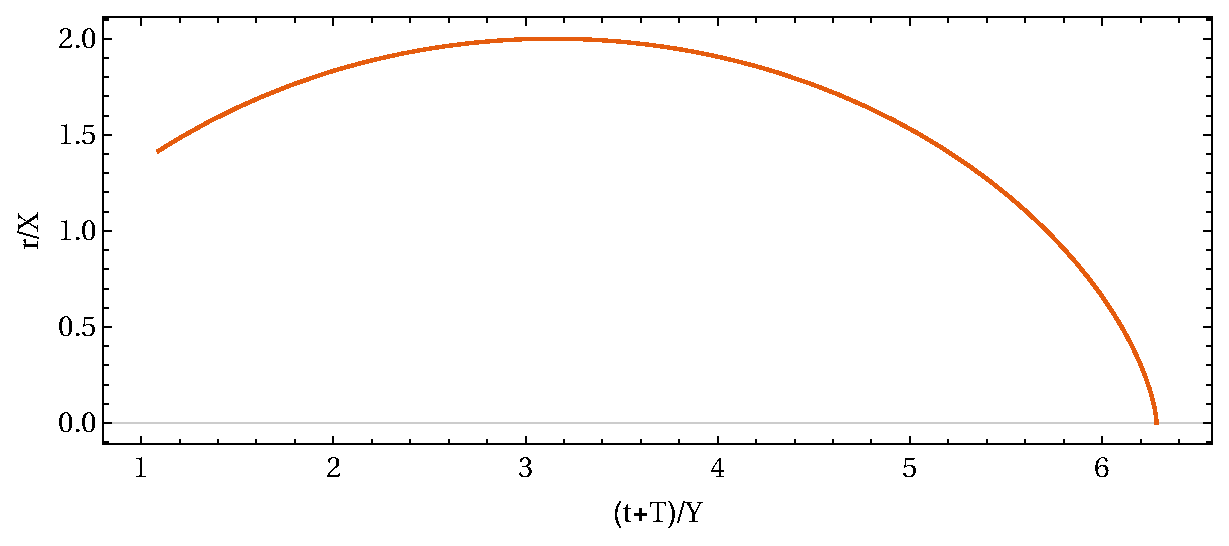
\includegraphics[width=0.7\textwidth]{spherical.eps}
		\caption{\footnotesize Evolution of a spherically overdense region.}
		\label{fig:sphere-cycloid}
	\end{figure}
	Of course, collapse stops before $r=0$ because of pressure generated by fluid. The system \textbf{virializes} and comes to a halt at $r=r_{max}/2$ with a density of $170\rho_b(t_{coll})$ in a matter dominated universe. 
\end{frame}
\subsection{Halo mass function}
	\begin{frame}{Halo mass function: Beyond Press-Schechter}
		\begin{columns}
			\begin{column}{0.45\textwidth}
				\small The Millennium simulations showed the errors in the Press-Schechter halo mass function (HMF). A general HMF could be defined as
				\begin{block}{Sheth-Tormen Fitting function}
					\begin{equation}
					\begin{aligned}
					\frac{dn}{dM}&=-f(\sigma)\frac{\rho_m}{M}\frac{d\log\sigma}{dM}\\
					f(\sigma)&= A\left[\left(\frac{\sigma}{b}\right)^{-a}+1\right]e^{-c/\sigma^2}
					\end{aligned}
					\end{equation}
				\end{block}
				\begin{itemize}
					\item $\rho_m$: Mean background density
					\item $\sigma$: Std. dev. of linear power spectrum
				\end{itemize}
			\end{column}
			\begin{column}{0.5\textwidth}
				\begin{figure}
					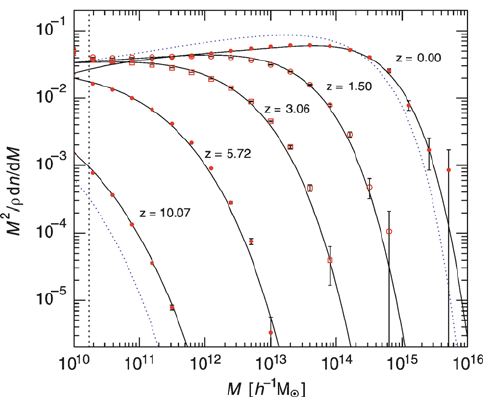
\includegraphics[width=\textwidth]{mill-hmf.png}
					\caption{\tiny Results from the Millennium simulation. The dotted line represents Press-Schechter. \emph{Source: Schneider, Extragalactic Astronomy and Cosmology, Ch. 7, Fig. 7.10}}
					\label{fig:mill-sim}
				\end{figure}
			\end{column}
		\end{columns}
	\end{frame}
\section{Data Analysis and Modelling}
	\subsection{Observed distribution of Absorbers}
		\begin{frame}{Observed distribution}
			\begin{figure}
				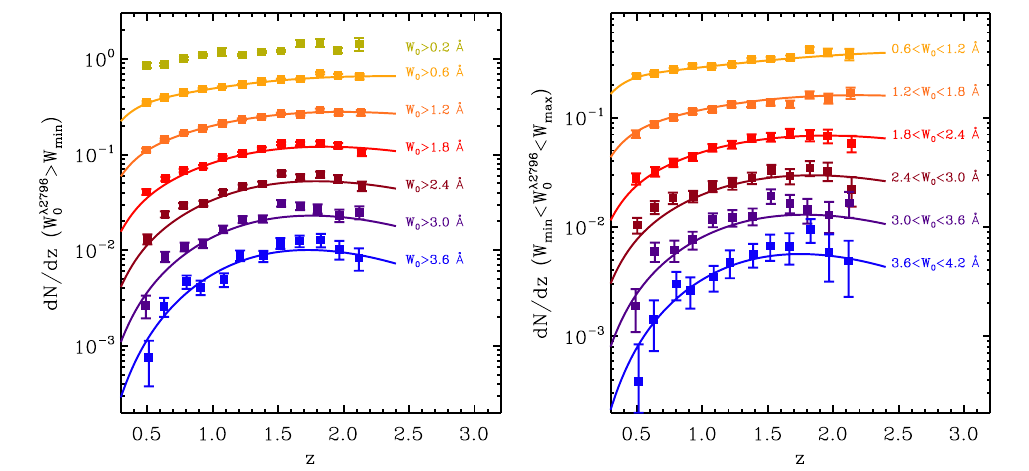
\includegraphics[width=\textwidth]{obs-distrib.png}
				\caption{\tiny  Cumulative (left) and differential (right) incidence rates dN/dz of Mg II absorbers. The solid lines show the best-fit parametrisation. The	redshift evolution is much stronger for stronger absorbers. \emph{Source: Zhu-Menard 2013, ApJ 770:130}}
				\label{fig:Zhu-Men13}
			\end{figure}
		\end{frame}
	\subsection{Modelling the absorber distribution}
		\begin{frame}{Halo-Absorber model: Tinker \& Chen 2008}
			\begin{columns}
				\begin{column}{0.5\textwidth}
					\begin{figure}
						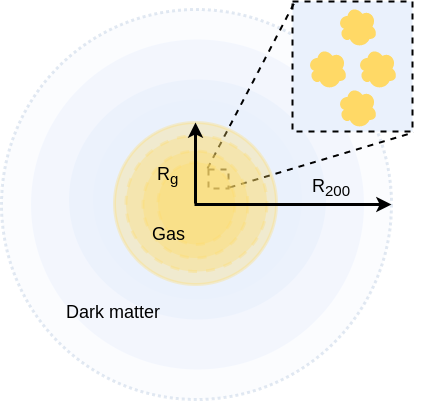
\includegraphics[width=\textwidth]{halo-model.png}
						\caption{\tiny The classical model proposed by Tinker and Chen 2008, ApJ 679:1218}
					\end{figure}
				\end{column}
				\begin{column}{0.5\textwidth}
					\begin{block}{Halo-Absorber model}
						Halo: Has \textbf{NFW mass} profile. Radius defined through:
						$$
							M=200\rho_m\frac{4}{3}\pi R_{200}^3
						$$
						Gas: Arranged in clumps within $R_g$. Distribution of clumps is of the form:
						$$
						\begin{aligned}
							\rho_g &= f_gG_0/(r^2+a_h^2)\\
							G_0 &= \frac{M(<R_g)/4\pi}{R_g-a_h\arctan(R_g/a_h)}\\
						\end{aligned}
						$$
					\end{block}
				\end{column}
			\end{columns}
		\end{frame}
		\begin{frame}{Probability density of REW}
			\begin{columns}
				\begin{column}{0.4\textwidth}
					\begin{figure}
						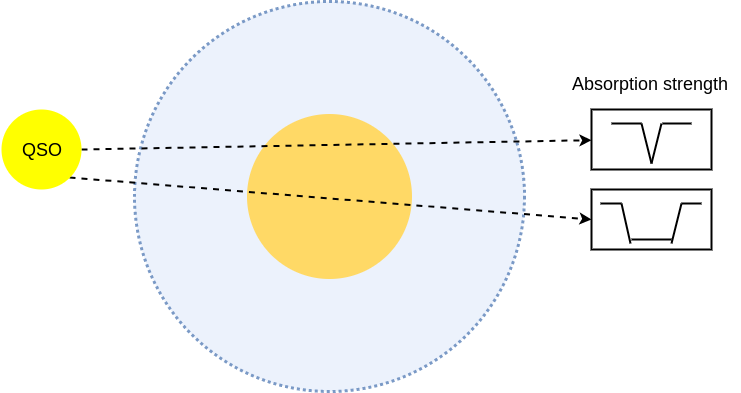
\includegraphics[width=\textwidth]{halo-absorb.png}
						\caption{\tiny Absorption strength depends on impact parameter and gas distribution properties}
						\label{fig:halo-absorb}
					\end{figure}
				\end{column}
				\begin{column}{0.6\textwidth}
					\begin{block}{REW vs impact parameter}
						\small{						$$
						\begin{aligned}
						W_r(s|M)&=\frac{W_0\sigma_{cl}f_g}{M_{cl}}\frac{2G_0}{\sqrt{s^2+a_h^2}}\times\\
						&\arctan{\frac{R_g^2-s^2}{s^2+a_h^2}}\\
						&=A_w\frac{2G_0}{\sqrt{s^2+a_h^2}}\arctan{\frac{R_g^2-s^2}{s^2+a_h^2}}
						\end{aligned}
						$$
					}
					\end{block}
					\begin{equation}
					\small{
						\begin{aligned}
							P(W_r|M)dW_r=\kappa_g(M)P(s|M)ds\\
							P(W_r|M)=\kappa_g(M)\frac{2s(W_r|M)}{R_g^2}\frac{ds}{dW_r}\\
						\end{aligned}
					}
					\end{equation}
				\end{column}
			\end{columns}
		\end{frame}
		\begin{frame}{Number density of absorbers}
			\begin{columns}
				\begin{column}{0.6\textwidth}
					\begin{block}{Absorber distribution}
						\begin{equation}
						\begin{aligned}
						\frac{d^2N}{dW_rdl}=\int dM&\times\text{Number density of halos}\\
						&\times\text{Total cross section}\\
						&\times P(W_r|M)\\
						\end{aligned}
						\end{equation}
						$$
						\begin{aligned}
						\frac{d^2N}{dW_rdl}&=\int dM\frac{dN}{dM}\pi R_g^2P(W_r|M)\\
						\frac{dN}{dz}&=\frac{dl}{dz}\int dW_r\frac{d^2N}{dW_rdl}\\
						\end{aligned}
						$$
					\end{block}
				\end{column}
				\begin{column}{0.3\textwidth}
					\begin{block}{Current state of work}
						\begin{itemize}
							\item Speeding up the integral for $d^2N/dW_rdl$
							\item Checking for numerical errors
						\end{itemize}
						Currently, computed $dN/dz$ is a decreasing function of redshift, unlike Zhu-Menard's observations.
					\end{block}
				\end{column}
			\end{columns}
		\end{frame}
\section{References}
		\begin{frame}{References}
			\begin{enumerate}
				\item \textbf{Zhu, Menard},\textit{The JHU-SDSS Metal Absorption Line Catalogue}, The Astrophysical Journal, 770:130 (15pp), 2013 June 20
				\item \textbf{Tinker, Chen}, \textit{On the Halo Occupation of Dark Baryons}, The Astrophysical Journal, 679:1218-1231, 2008
				\item \textbf{T. Padmanabhan}, \textit{Structure formation in the universe}, Cambridge 1993
				\item \textbf{Jim Peebles}, \textit{Large Scale Structure of the Universe}, Princeton 1992
				\item \textbf{Peter Schneider}, \textit{Extragalactic Astronomy and Cosmology}, Springer 2006
			\end{enumerate}
		\end{frame}
\end{document}